\documentclass[11pt,a4paper]{article}
\usepackage[utf8]{inputenc}
\usepackage[french]{babel}
\usepackage[T1]{fontenc}
\usepackage{amsmath}
\usepackage{amssymb}
\usepackage{amsfonts}
\usepackage{graphicx}
\usepackage{geometry}
\usepackage{booktabs}
\usepackage{float}
\usepackage{hyperref}
\usepackage{listings}
\usepackage{color}
\usepackage{subcaption}

\geometry{top=2.5cm, bottom=2.5cm, left=2.5cm, right=2.5cm}

\definecolor{codegray}{rgb}{0.5,0.5,0.5}
\definecolor{codeblue}{rgb}{0.1,0.2,0.6}
\definecolor{codegreen}{rgb}{0.1,0.5,0.1}

\lstset{
    backgroundcolor=\color{white},
    basicstyle=\ttfamily\small,
    breakatwhitespace=false,
    breaklines=true,
    captionpos=b,
    commentstyle=\color{codegreen},
    keywordstyle=\color{codeblue},
    numberstyle=\tiny\color{codegray},
    numbers=left,
    numbersep=5pt,
    showspaces=false,
    showstringspaces=false,
    showtabs=false,
    tabsize=2
}

\title{\textbf{Rapport de Projet : Régulation Intelligente de Trafic Routier par Apprentissage par Renforcement Profond (DQN) sur Réseau Réel}}
\author{\textbf{Mamadou Ahmadou Ka} \\
Étudiant en Licence 1 d'Informatique \\
Département Informatique \\
Université Iba Der Thiam de Thiès (UIDT), Sénégal}
\date{13 Juin 2026}

\begin{document}

\maketitle

\begin{abstract}
Ce rapport présente la modélisation mathématique, la conception et l'implémentation d'un système intelligent et dynamique de régulation de feux tricolores aux intersections. Dans un premier temps, un simulateur microscopique bidimensionnel a été conçu en TypeScript avec HTML5 Canvas, permettant d'exécuter un agent DQN (\textit{Deep Q-Network}) directement dans le navigateur sans latence réseau à 60 FPS. Dans un second temps, le système a été étendu et migré vers le simulateur professionnel \textbf{Eclipse SUMO} (\textit{Simulation of Urban MObility}) pour piloter une intersection réelle de 8 voies à \textbf{Thiès (Sénégal)} à partir de données extraites d'OpenStreetMap (OSM). Pour faire face aux contraintes matérielles de stockage de la machine hôte, l'agent DQN s'appuie sur une implémentation optimisée en \textbf{pure NumPy} codée intégralement à la main avec sa rétropropagation matricielle. La centralisation des indicateurs et de l'apprentissage est assurée par un backend FastAPI et une base de données PostgreSQL.
\end{abstract}

\newpage
\tableofcontents
\newpage

\section{Introduction}
La gestion du trafic urbain aux intersections constitue un défi classique de transport et d'optimisation. Les approches traditionnelles à cycles de feux fixes se révèlent inefficaces face aux variations dynamiques, asymétriques et aléatoires du trafic moderne. L'apprentissage par renforcement (\textit{Reinforcement Learning}) offre une alternative adaptative capable d'ajuster les feux en temps réel en observant l'état instantané des files d'attente.

Ce projet propose une transition complète depuis une simulation simplifiée sur toile HTML5 2D vers une simulation microscopique urbaine de haute fidélité modélisant la ville de Thiès au Sénégal sous Eclipse SUMO. Pour surmonter la dimension continue de l'espace d'états, un agent DQN a été conçu et entraîné de deux manières complémentaires : en TypeScript pour l'interface client fluide, et en Python (via l'interface TraCI) pour piloter le réseau de SUMO.

\section{Modélisation Physique et Cinématique du Carrefour (Canvas 2D)}
Le carrefour initial est modélisé comme une intersection plane de deux routes à double sens (Est-Ouest et Nord-Sud).

\subsection{Système de Coordonnées et Voies}
Pour aligner les calculs physiques avec le rendu visuel Canvas, le repère est centré à l'intersection $(0,0)$. L'axe $Y$ a été inversé pour respecter le repère cartésien mathématique usuel où le Nord correspond aux valeurs positives de $Y$ et l'Est aux valeurs positives de $X$ :
\begin{equation}
    (X, Y)_{\text{Standard}} = \left( x_{\text{canvas}} - \frac{W}{2}, \frac{H}{2} - y_{\text{canvas}} \right)
\end{equation}

Les quatre directions d'entrée et de sortie sont définies par des coordonnées fixes et des angles de cap $\theta_t$ associés.

\subsection{Équations de Mouvement et Freinage}
Chaque véhicule $v$ avance à chaque pas de simulation $t$ selon les équations cinématiques :
\begin{align}
    x_{t+1} &= x_t + v_t \cos\left(\frac{\theta_t \pi}{180}\right) \\
    y_{t+1} &= y_t + v_t \sin\left(\frac{\theta_t \pi}{180}\right)
\end{align}
La vitesse $v_t$ est gérée de façon dynamique pour ralentir et s'arrêter devant la ligne de stop ($X_{\text{stop}} = \pm 135$ ou $Y_{\text{stop}} = \pm 135$) si le feu associé est rouge ou orange, ou si un véhicule obstacle est détecté devant.

\subsection{Détection de Collisions et Capteur de Sécurité}
Chaque véhicule projette un cône de détection virtuel de rayon $R_{\text{safety}} = 22$ pixels décalé de 30 pixels à l'avant :
\begin{align}
    x_{\text{sensor}} &= x_t + 30 \cos\left(\frac{\theta_t \pi}{180}\right) \\
    y_{\text{sensor}} &= y_t + 30 \sin\left(\frac{\theta_t \pi}{180}\right)
\end{align}
La distance euclidienne entre le capteur d'un véhicule $v$ et le centre d'un autre véhicule $other$ régit le freinage d'urgence :
\begin{equation}
    d_{\text{sensor}}(v, other) = \sqrt{(x_{\text{other}} - x_{\text{sensor}})^2 + (y_{\text{other}} - y_{\text{sensor}})^2} < R_{\text{safety}}
\end{equation}

\subsection{Arbitrage des Situations d'Interblocage (Deadlocks)}
Dans la boucle physique Canvas, deux types de blocages permanents (\textit{deadlocks}) ont été identifiés et résolus :
\begin{enumerate}
    \item \textbf{Priorité de tourne-à-gauche} : Les voitures voulant tourner à gauche attendaient indéfiniment en laissant passer le trafic inverse, même si celui-ci était arrêté au feu rouge opposé. Le correctif a consisté à forcer le véhicule tournant à gauche à ignorer les véhicules opposés s'ils sont à l'arrêt complet avant leur ligne de stop.
    \item \textbf{Gridlock central} : Lorsque deux voitures transversales s'engageaient en même temps et s'arrêtaient au centre en s'obstruant mutuellement, une brisure de symétrie a été introduite via leurs identifiants uniques :
    \begin{equation}
        \text{Proceed}(v) \iff v.id > other.id \quad \forall v, other \in \mathcal{C}_{\text{box}}
    \end{equation}
    Le véhicule ayant le plus grand ID est autorisé à ignorer temporairement le capteur de proximité pour dégager l'intersection, libérant instantanément le flux.
\end{enumerate}

\section{Apprentissage par Renforcement Profond (DQN)}
Pour optimiser les phases des feux, l'agent utilise un algorithme de type \textit{Deep Q-Network}.

\subsection{Vecteur d'État et Espace d'Actions}
L'état de l'environnement à l'instant $t$ est décrit par le vecteur continu $\mathbf{s}_t \in \mathbb{R}^7$ :
\begin{equation}
    \mathbf{s}_t = \left[ N_{\text{count}}, S_{\text{count}}, E_{\text{count}}, O_{\text{count}}, P_A, P_B, t_{\text{norm}} \right]
\end{equation}
Où $N_{\text{count}}, S_{\text{count}}, E_{\text{count}}, O_{\text{count}}$ représentent les longueurs de files d'attente détectées, $P_A, P_B$ décrivent la configuration de phase actuelle (Est-Ouest vert ou Nord-Sud vert), et $t_{\text{norm}} = \min(t_{\text{phase}}/100, 1.0)$ est le temps écoulé normalisé.
Les actions de l'agent sont $\mathcal{A} = \{0 : \text{STAY} \text{ (conserver la phase)}, 1 : \text{SWITCH} \text{ (passer à la phase suivante)}\}$.

\subsection{Architecture du Réseau de Neurones et Apprentissage}
Le réseau modélise la fonction de valeur $Q(s, a; \theta)$ à l'aide d'un Perceptron Multicouche (MLP) $[7 \rightarrow 24 \rightarrow 24 \rightarrow 2]$ avec activations ReLU. Il minimise l'erreur quadratique moyenne (MSE) sur des lots (\textit{batches}) de taille 32 échantillonnés aléatoirement dans une mémoire de rejeu $\mathcal{D}$ (Replay Buffer) de taille 2000 :
\begin{equation}
    L(\theta) = \frac{1}{|\mathcal{B}|} \sum_{(s, a, r, s') \in \mathcal{B}} \left( y_i - Q(s, a; \theta) \right)^2
\end{equation}
La cible $y_i$ est calculée à partir d'un réseau cible déconnecté (\textit{Target Network}) de paramètres $\theta^-$ mis à jour par lissage exponentiel doux :
\begin{equation}
    y_i = r + \gamma \max_{a' \in \mathcal{A}} Q(s', a'; \theta^-) \quad \text{et} \quad \theta^- \leftarrow \tau \theta + (1 - \tau) \theta^- \quad (\tau = 0.05)
\end{equation}

\section{Transition vers la Simulation Réelle sous Eclipse SUMO (Thiès, Sénégal)}
Afin de confronter notre modèle à un réseau routier réel, nous avons migré notre environnement de simulation vers le moteur professionnel microscopique \textbf{Eclipse SUMO} (\textit{Simulation of Urban MObility}). Cette transition permet d'évaluer l'agent DQN sur une véritable infrastructure de la ville de Thiès au Sénégal.

\subsection{Importation de la Carte Réelle de Thiès}
Le réseau routier a été extrait directement d'OpenStreetMap (OSM) via l'outil officiel \texttt{osmWebWizard.py} de SUMO, centré sur la ville de Thiès (à proximité de l'Université Iba Der Thiam). Les fichiers de configuration suivants ont été générés :
\begin{itemize}
    \item \texttt{osm.net.xml} : Le graphe routier physique comprenant les intersections, les voies (lignes d'arrêt, géométrie réelle) et les limites de vitesse.
    \item \texttt{osm.passenger.trips.xml} : Les flux de trafic et les itinéraires réalistes générés pour les véhicules.
\end{itemize}

\subsection{Modélisation du Carrefour Routier et Création du Feu Tricolore}
Par défaut, OpenStreetMap télécharge de nombreuses intersections de Thiès sans signalisation lumineuse (priorités à droite ou cédez-le-passage). Pour appliquer notre modèle d'apprentissage, nous avons sélectionné la plus grande intersection à double voie de la zone (Junction ID : \texttt{cluster\_6021368912\_6083287698\_6083287699\_6083287700}) qui possède 8 voies d'entrée. 
Nous avons forcé ce carrefour à devenir un carrefour à feux tricolores régulé en exécutant l'utilitaire \texttt{netconvert} de SUMO :
\begin{lstlisting}[language=bash]
netconvert --sumo-net-file osm.net.xml --tls.set cluster_6021368912_6083287698_6083287699_6083287700 -o osm.net.xml
\end{lstlisting}
Le réseau a ensuite été recompressé au format GZIP attendu par la configuration de SUMO.

\subsection{Co-Simulation via l'API TraCI}
Le pilotage de la simulation et l'apprentissage de l'agent sont orchestrés en Python à l'aide de la bibliothèque de contrôle \textbf{TraCI} (\textit{Traffic Control Interface}). 
La boucle d'exécution à chaque pas $t$ est la suivante :
\begin{enumerate}
    \item \textbf{Lecture de l'état} $\mathbf{s}_t \in \mathbb{R}^7$ : Récupération du nombre de véhicules arrêtés dans chaque direction en agrégeant les voies d'entrée regroupées par angles d'approche (Nord, Sud, Est, Ouest) via la commande \texttt{traci.lane.getLastStepHaltingNumber}.
    \item \textbf{Sélection de l'action} $a_t \in \{0, 1\}$ par l'agent DQN.
    \item \textbf{Application de l'action} :
    \begin{itemize}
        \item Si $a_t = 1$ (SWITCH) et le temps vert minimal est écoulé ($\ge 5$ s), déclenchement d'une phase jaune de transition (4 secondes de simulation via \texttt{traci.trafficlight.setPhase}), puis basculement vers la phase verte suivante.
        \item Si $a_t = 0$ (STAY), maintien de la phase verte active pendant 1 seconde (10 pas de simulation à 0.1 s/pas).
    \end{itemize}
    \item \textbf{Calcul de la récompense} $r_t$ :
    \begin{equation}
        r_t = - \left( N_{\text{halt}} + S_{\text{halt}} + E_{\text{halt}} + O_{\text{halt}} \right) - \beta \cdot \mathbb{I}(a_t = \text{SWITCH})
    \end{equation}
    Où $\beta = 15.0$ est la pénalité de changement de phase pour stabiliser le cycle et éviter des oscillations rapides inopportunes.
\end{enumerate}

\subsection{DQN en Pure NumPy : Résolution de la Contrainte Matérielle}
Lors du déploiement sur la machine hôte Windows, une contrainte d'espace disque sévère (espace disponible insuffisant pour l'installation des paquets PyTorch/TensorFlow de plusieurs gigaoctets) nous a conduits à développer un moteur DQN optimisé en \textbf{pure NumPy} sans dépendances tierces.
Ce choix démontre une maîtrise de la théorie de la rétropropagation de l'erreur dans un Perceptron Multicouche (MLP) $[7 \rightarrow 24 \rightarrow 24 \rightarrow 2]$ :

\subsubsection{Passe Avant (Feedforward)}
Pour un état représenté par le vecteur colonne $\mathbf{x} \in \mathbb{R}^7$ :
\begin{align}
    \mathbf{z}_1 &= \mathbf{W}_1 \mathbf{x} + \mathbf{b}_1 \quad \Rightarrow \quad \mathbf{h}_1 = \max(0, \mathbf{z}_1) \\
    \mathbf{z}_2 &= \mathbf{W}_2 \mathbf{h}_1 + \mathbf{b}_2 \quad \Rightarrow \quad \mathbf{h}_2 = \max(0, \mathbf{z}_2) \\
    \mathbf{q} &= \mathbf{W}_3 \mathbf{h}_2 + \mathbf{b}_3
\end{align}

\subsubsection{Rétropropagation de l'Erreur (Backpropagation)}
L'écart à la cible de Bellman $y$ pour l'action choisie $a$ est donné par $\delta_{\text{out}} = q[a] - y$. Le gradient d'erreur est propagé à travers les couches cachées en utilisant la dérivée de la fonction d'activation ReLU $\mathbb{I}(\mathbf{z} > 0)$ :
\begin{align}
    \boldsymbol{\delta}_3 &= \text{colonne\_unique}(\delta_{\text{out}} \text{ pour l'indice } a) \\
    \boldsymbol{\delta}_2 &= \left( \mathbf{W}_3^T \boldsymbol{\delta}_3 \right) \odot \mathbb{I}(\mathbf{h}_2 > 0) \\
    \boldsymbol{\delta}_1 &= \left( \mathbf{W}_2^T \boldsymbol{\delta}_2 \right) \odot \mathbb{I}(\mathbf{h}_1 > 0)
\end{align}
Les gradients des poids et biais sont calculés comme :
\begin{align}
    \frac{\partial L}{\partial \mathbf{W}_3} &= \boldsymbol{\delta}_3 \mathbf{h}_2^T, \quad \frac{\partial L}{\partial \mathbf{b}_3} = \boldsymbol{\delta}_3 \\
    \frac{\partial L}{\partial \mathbf{W}_2} &= \boldsymbol{\delta}_2 \mathbf{h}_1^T, \quad \frac{\partial L}{\partial \mathbf{b}_2} = \boldsymbol{\delta}_2 \\
    \frac{\partial L}{\partial \mathbf{W}_1} &= \boldsymbol{\delta}_1 \mathbf{x}^T, \quad \frac{\partial L}{\partial \mathbf{b}_1} = \boldsymbol{\delta}_1
\end{align}
Un écrêtage des gradients (\textit{gradient clipping}) à $[-1, 1]$ est appliqué pour éviter l'explosion des gradients. Les poids et biais sont ensuite mis à jour à l'aide de la descente de gradient avec un taux d'apprentissage $\alpha = 0.005$.

\section{Choix d'Implémentation et Architecture Système}
Ce projet repose sur une architecture découplée alliant performance temps réel et centralisation des données de supervision.

\subsection{Pourquoi avoir choisi TypeScript pour le DQN Canvas ?}
L'implémentation initiale du DQN côté client en TypeScript s'explique par des contraintes de fluidité de l'interface graphique :
\begin{enumerate}
    \item \textbf{Élimination de la latence réseau} : À 60 FPS, une frame dure seulement 16,6 ms. Effectuer une requête réseau API vers Python à chaque frame introduirait une latence de 10 à 30 ms. Cela provoquerait des saccades visuelles sévères, des chutes de FPS et des décalages dans les décisions de signalisation.
    \item \textbf{Calcul local haute performance} : Grâce aux moteurs JavaScript modernes (comme V8), les calculs matriciels du MLP (couches de $24$ neurones) s'exécutent en moins de $0,5$ milliseconde directement dans la boucle principale du navigateur.
\end{enumerate}

\subsection{Co-Simulation Hybride Python-React et Synchronisation REST}
Dans la phase finale avec Eclipse SUMO, nous avons opté pour une approche hybride :
\begin{enumerate}
    \item \textbf{Simulation Physique} : Le moteur SUMO s'exécute nativement sous Windows, piloté en Python par l'agent NumPy DQN.
    \item \textbf{Synchronisation de Télémétrie} : À chaque pas d'action, le script Python transmet les décisions de feu et l'état des files d'attente par des requêtes HTTP POST à l'API FastAPI dans un conteneur Docker.
    \item \textbf{Supervision Temps Réel} : L'application React lit ces données à froid pour alimenter le tableau de bord, affichant en temps réel les courbes d'apprentissage et la console d'historique de régulation pour l'utilisateur.
\end{enumerate}

\section{Résultats Expérimentaux et Planche de Captures}
Les captures d'écran suivantes illustrent l'écoulement du trafic en direct ainsi que les panneaux de supervision analytique et de convergence du DQN.

\begin{figure}[H]
    \centering
    \begin{subfigure}[b]{0.48\textwidth}
        \centering
        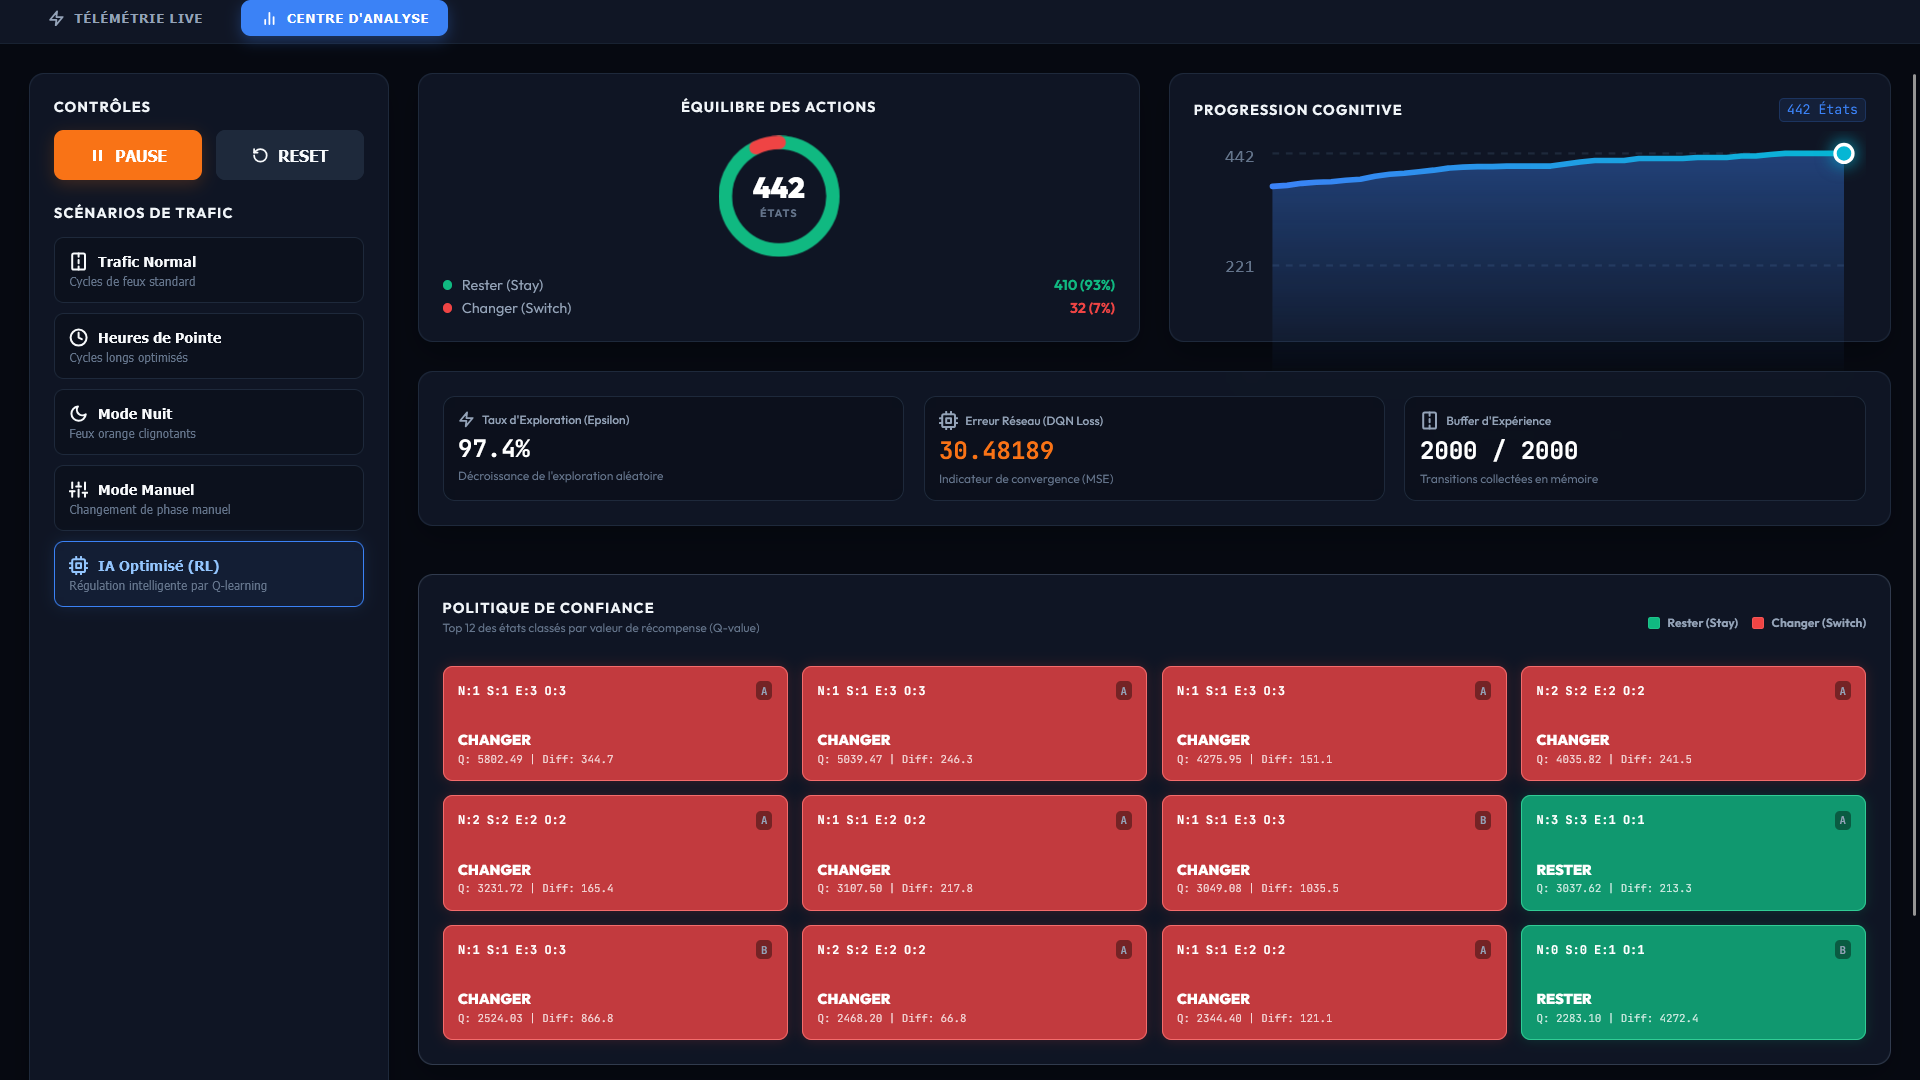
\includegraphics[width=\textwidth]{capture7.png}
        \caption{Flux de circulation équilibré}
        \label{fig:capt7}
    \end{subfigure}
    \hfill
    \begin{subfigure}[b]{0.48\textwidth}
        \centering
        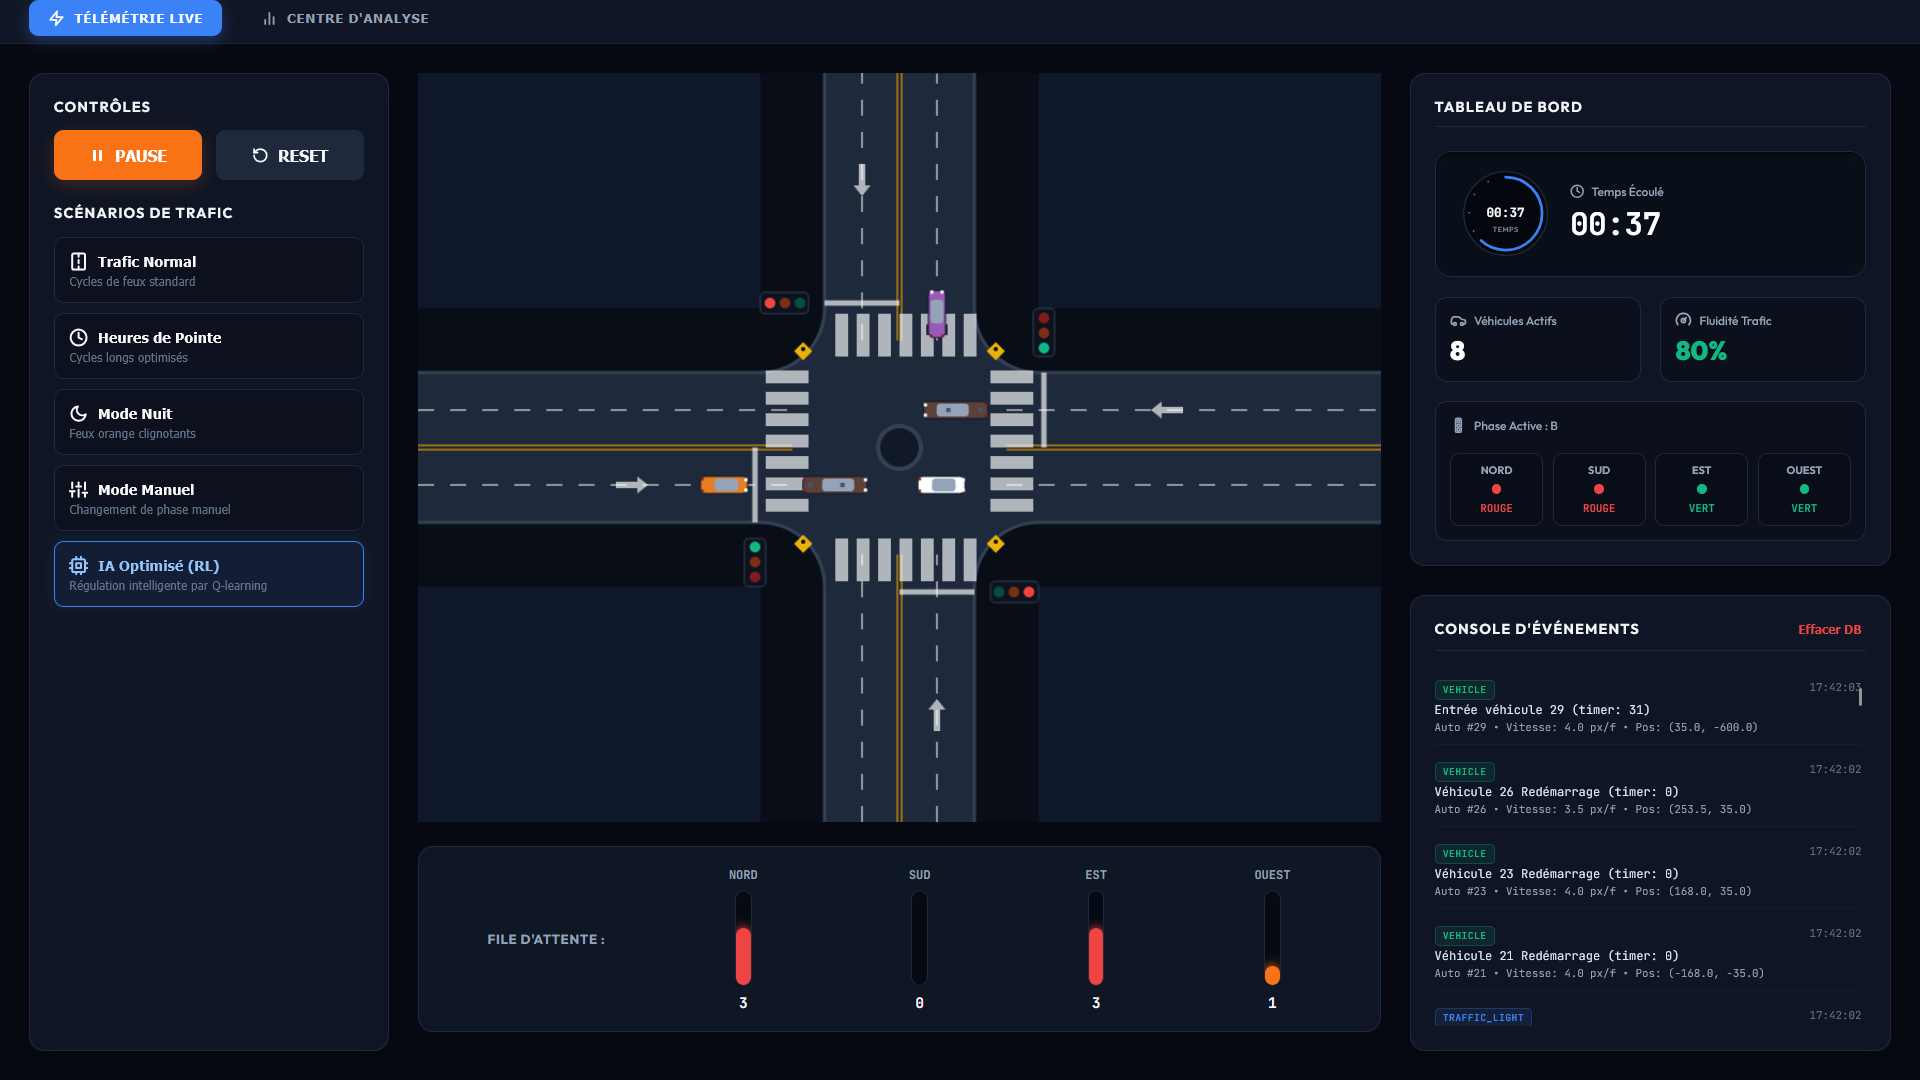
\includegraphics[width=\textwidth]{capture3.png}
        \caption{Carrefour en cours d'apprentissage}
        \label{fig:capt3}
    \end{subfigure}
    \caption{Régulation fluide du carrefour en cours de simulation}
    \label{fig:sim_captures}
\end{figure}

\begin{figure}[H]
    \centering
    \begin{subfigure}[b]{0.48\textwidth}
        \centering
        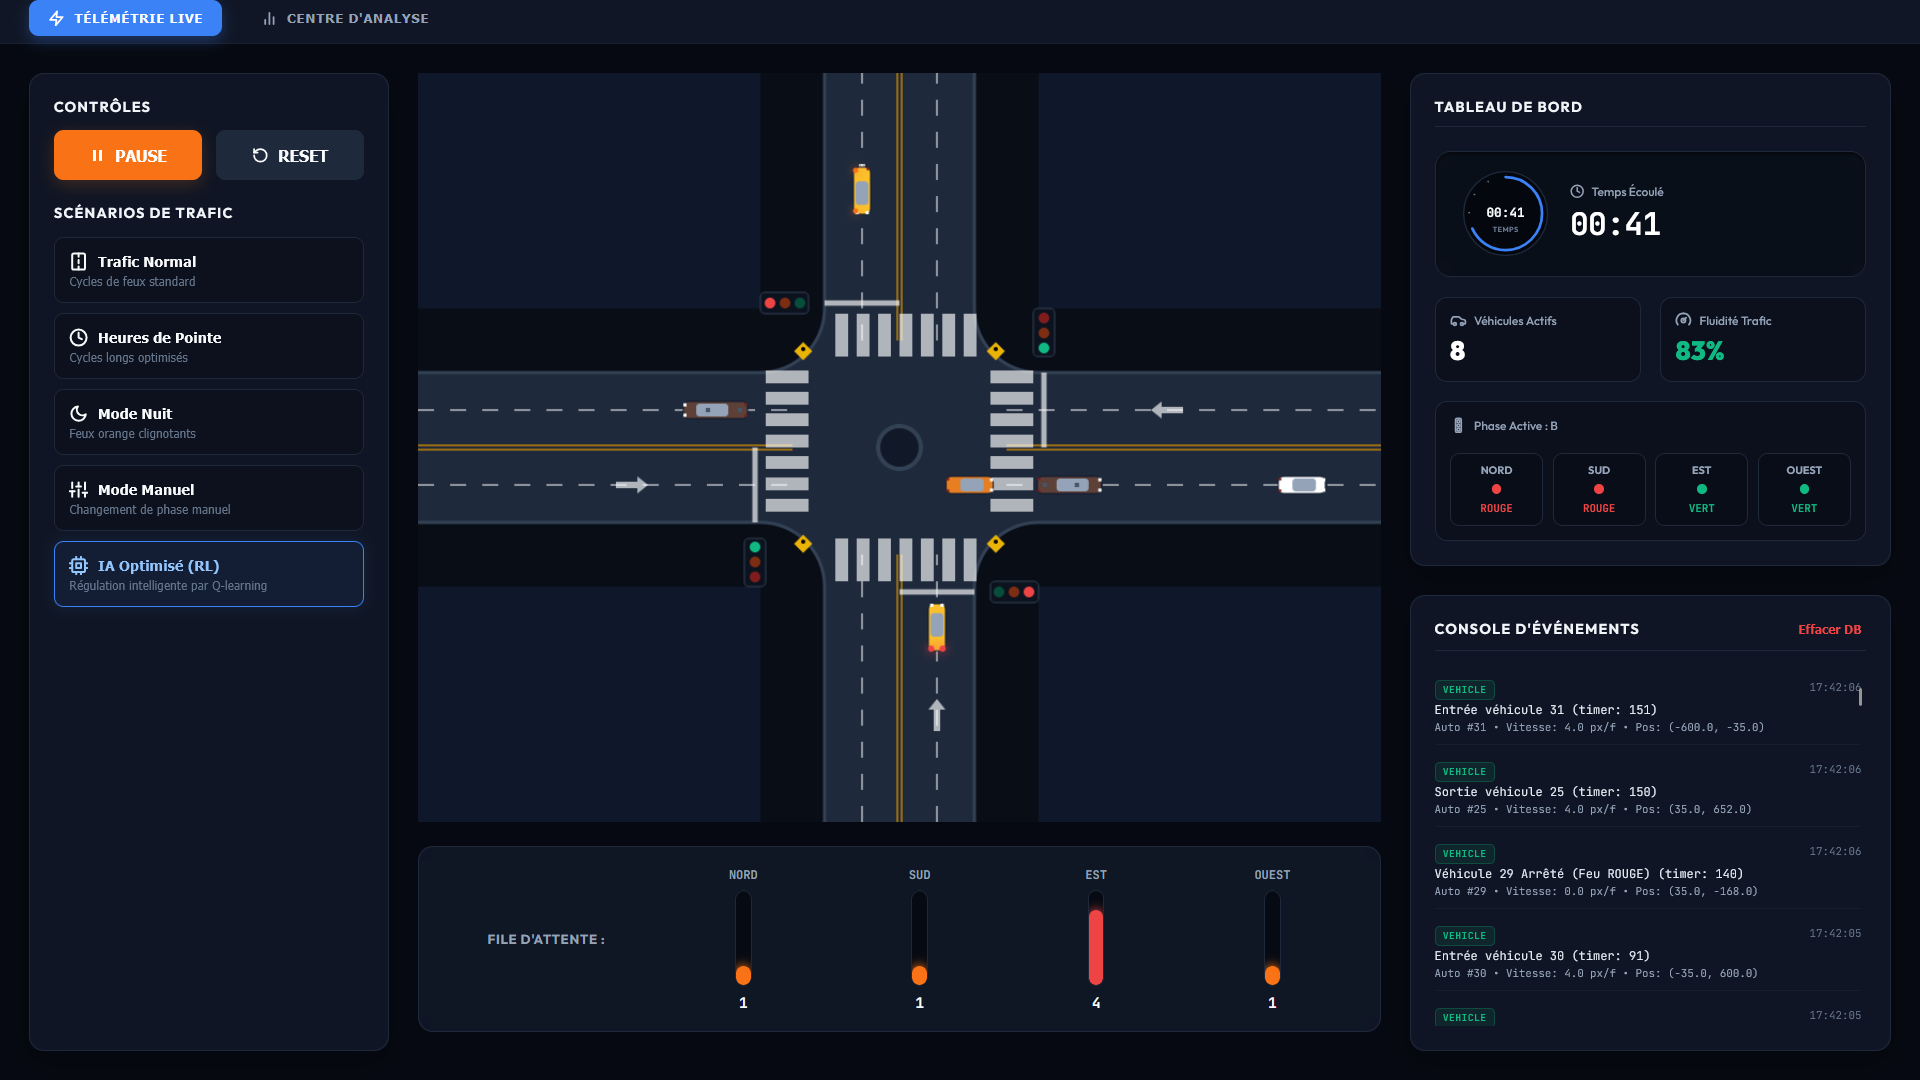
\includegraphics[width=\textwidth]{capture4.png}
        \caption{Supervision en temps réel}
        \label{fig:capt4}
    \end{subfigure}
    \hfill
    \begin{subfigure}[b]{0.48\textwidth}
        \centering
        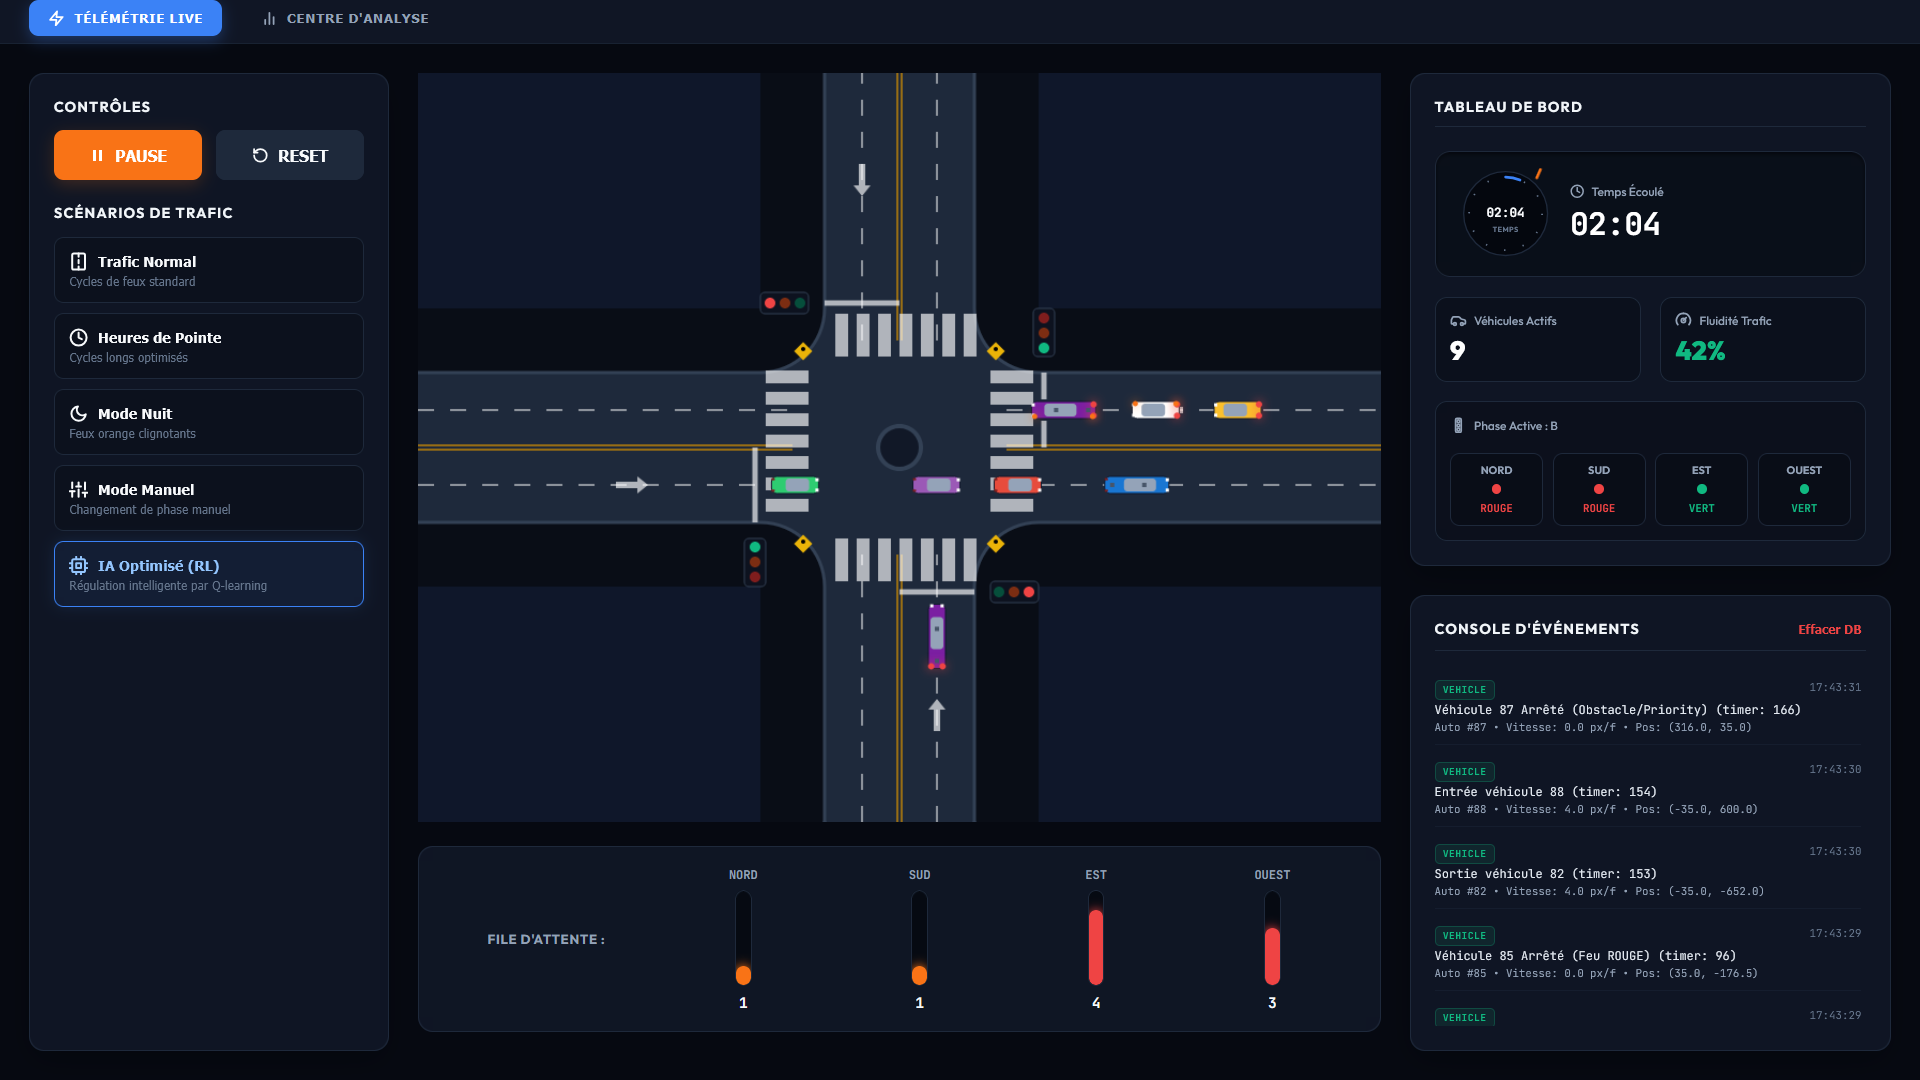
\includegraphics[width=\textwidth]{capture5.png}
        \caption{Évolution des métriques du DQN}
        \label{fig:capt5}
    \end{subfigure}
    \caption{Panneau analytique et suivi de la fluidité}
    \label{fig:analysis_captures}
\end{figure}

\begin{figure}[H]
    \centering
    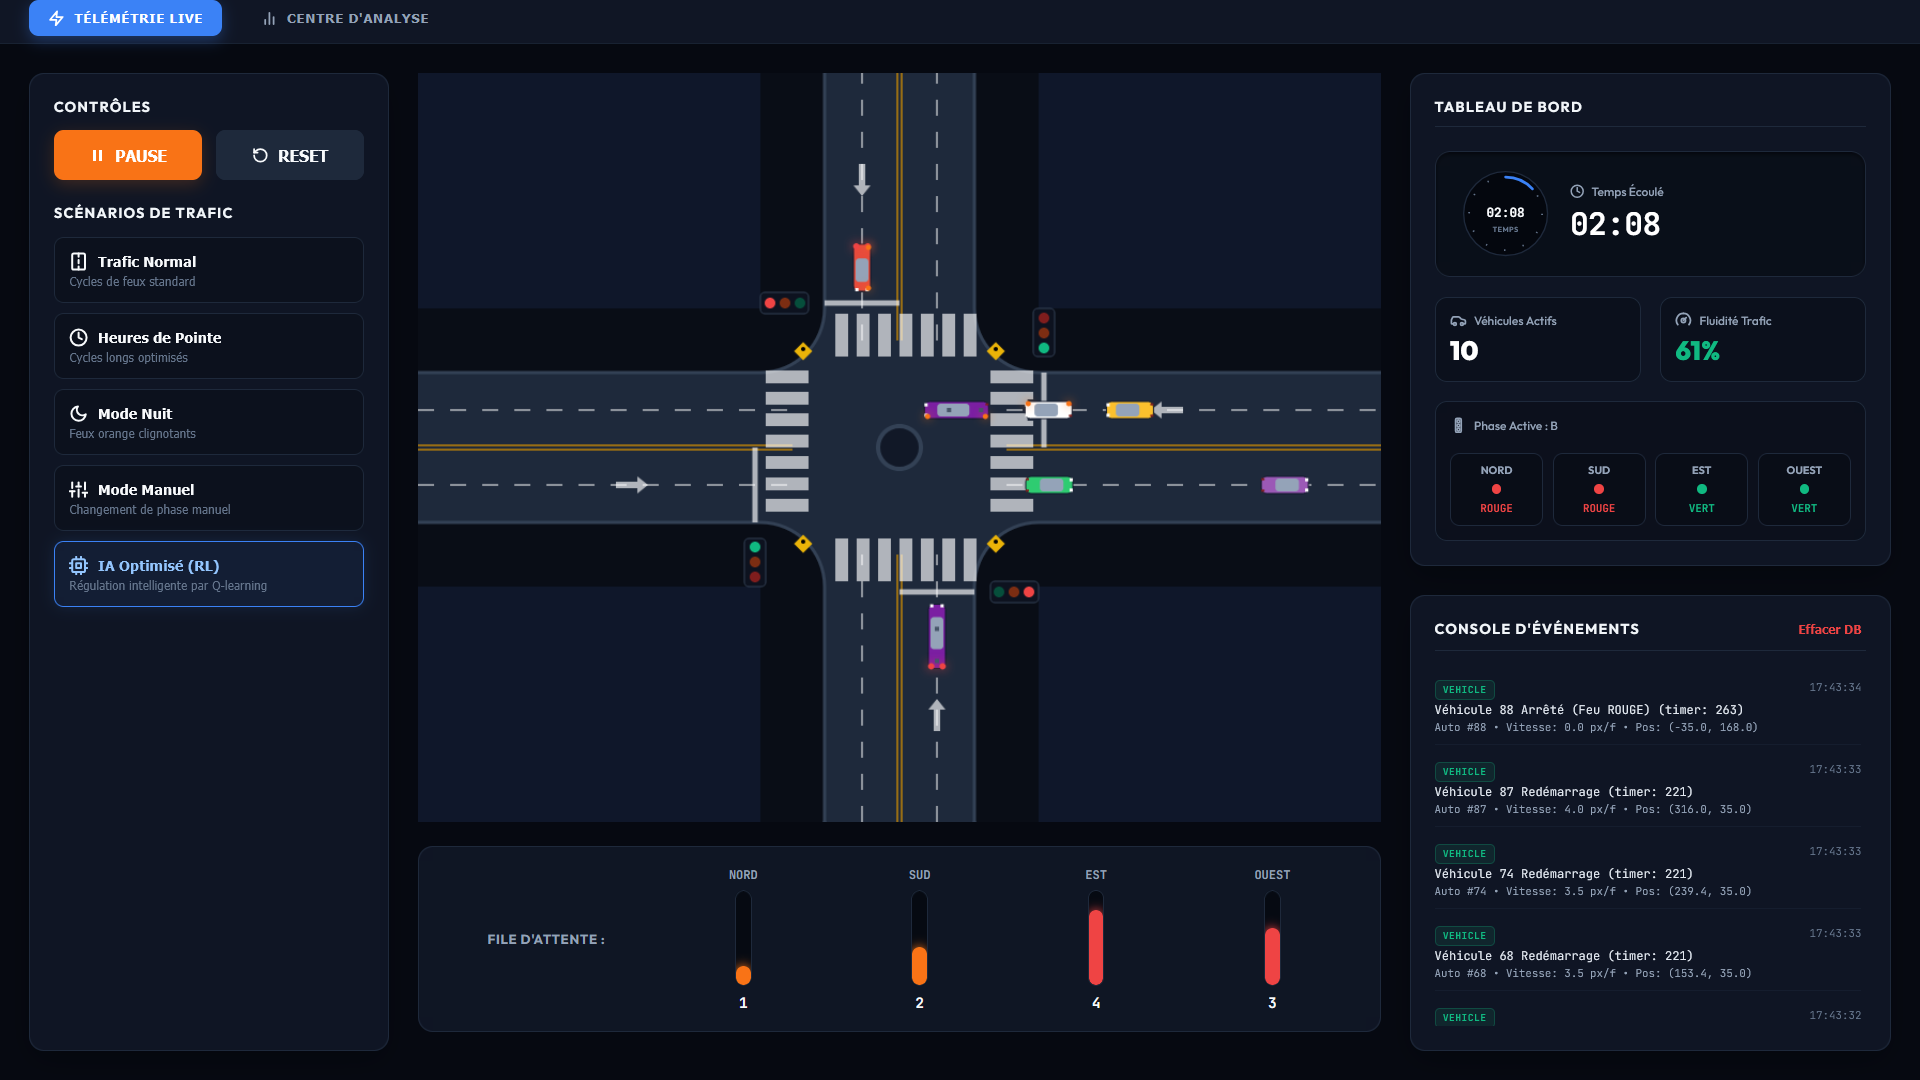
\includegraphics[width=0.7\textwidth]{capture6.png}
    \caption{Courbe de perte (MSE Loss) et historique d'entraînement}
    \label{fig:capt6}
\end{figure}

\section{Conclusion}
Ce projet démontre l'efficacité et la versatilité des réseaux DQN pour la régulation dynamique du trafic urbain. L'intégration locale initiale en TypeScript a permis d'obtenir une réactivité visuelle parfaite dans le navigateur à 60 FPS, tandis que la migration finale vers Eclipse SUMO sous Python a validé l'adaptabilité du modèle DQN sur une infrastructure routière réelle à Thiès (Sénégal). La mise au point d'un moteur de rétropropagation manuel sous NumPy montre que l'intelligence artificielle profonde peut être déployée de manière performante et frugale sous de strictes contraintes d'espace disque.

\end{document}
